%%%%%%%%%%%%%%%%%%%%%%%%%%%%%%%%%%%%%%%%%
% Stylish Article
% LaTeX Template
% Version 2.2 (2020-10-22)
%
% This template has been downloaded from:
% http://www.LaTeXTemplates.com
%
% Original author:
% Mathias Legrand (legrand.mathias@gmail.com) 
% With extensive modifications by:
% Vel (vel@latextemplates.com)
%
% License:
% CC BY-NC-SA 3.0 (http://creativecommons.org/licenses/by-nc-sa/3.0/)
%
%%%%%%%%%%%%%%%%%%%%%%%%%%%%%%%%%%%%%%%%%

%----------------------------------------------------------------------------------------
%	PACKAGES AND OTHER DOCUMENT CONFIGURATIONS
%----------------------------------------------------------------------------------------

\documentclass[10pt]{SelfArx} % Document font size

\usepackage[T1]{fontenc} %font asked by Overleaf
\usepackage[french]{babel} % Specify a language

\usepackage[linesnumbered,ruled,vlined]{algorithm2e}

%%% Coloring the comment as blue
\newcommand\mycommfont[1]{\footnotesize\ttfamily\textcolor{blue}{#1}}
\SetCommentSty{mycommfont}

\SetKwInput{KwInput}{Input}                % Set the Input
\SetKwInput{KwOutput}{Output}              % set the Output

%----------------------------------------------------------------------------------------
%	COLUMNS
%----------------------------------------------------------------------------------------

\setlength{\columnsep}{0.55cm} % Distance between the two columns of text
\setlength{\fboxrule}{0.75pt} % Width of the border around the abstract

%----------------------------------------------------------------------------------------
%	COLORS
%----------------------------------------------------------------------------------------

\definecolor{color1}{RGB}{0,0,90} % Color of the article title and sections
\definecolor{color2}{RGB}{0,20,20} % Color of the boxes behind the abstract and headings

%----------------------------------------------------------------------------------------
%	HYPERLINKS
%----------------------------------------------------------------------------------------

\usepackage{hyperref} % Required for hyperlinks

\hypersetup{
	hidelinks,
	colorlinks,
	breaklinks=true,
	urlcolor=color2,
	citecolor=color1,
	linkcolor=color1,
	bookmarksopen=false,
	pdftitle={Title},
	pdfauthor={Author},
}

%----------------------------------------------------------------------------------------
%	ARTICLE INFORMATION
%----------------------------------------------------------------------------------------

\JournalInfo{IMT Atlantique, 14-06-2022} % Journal information
\Archive{CODEV Recherche} % Additional notes (e.g. copyright, DOI, review/research article)

\PaperTitle{Blocked Adaptive Cross Approximation (BACA)} % Article title

\Authors{KANIT Zaccarie \textsuperscript{1}*} % Authors
\affiliation{\textsuperscript{1}\textit{Étudiant en cycle d'ingénieur généraliste, IMT Atlantique}} % Author affiliation
\affiliation{*\textbf{mail}: zaccarie.kanit@imt-atlantique.net} % Corresponding author

\Keywords{Algorithme de résolution rapide -- (ML/B) ACA--Calcul Matriciel} % Keywords - if you don't want any simply remove all the text between the curly brackets
\newcommand{\keywordname}{Mots clés} % Defines the keywords heading name

%----------------------------------------------------------------------------------------
%	ABSTRACT
%----------------------------------------------------------------------------------------

\Abstract{Ce papier présente une variante de l'algorithme de calcul matricielle par ACA qui a pour objectif de réduire le temps de calcul et l'espace mémoire de la résolution des problèmes de nature électromagnétiques par la Méthode des Moments. L'algorithme proposé ici pour accélérer le calcul est l'approximation par bloc(BACA), une solution purement algébrique, qui remplace la solution par niveaux(MLACA) qui possède un manque de scalabilité. L'algorithme par bloc repose sur l'utilisation de la décomposition QR sur plus petites matrices pour améliorer la complexité. La convergence se fait donc plus rapidement et la qualité première de la ACA est maintenu; c'est à dire que l'algorithme étant purement algébrique est indépendant du noyau de Green tant que les matrices ont une déficience de rang. De plus,cet algorithme peut encore être optimisée grâce à la parallélisation (H-BACA) de l'algorithme par bloc. Celui-ci étant scalable en multi coeurs et donc diminuant le temps de compilation, en particulier pour les matrices sparses.}

%----------------------------------------------------------------------------------------

\begin{document}


\maketitle % Output the title and abstract box

\tableofcontents % Output the contents section

\thispagestyle{empty} % Removes page numbering from the first page

%----------------------------------------------------------------------------------------
%	ARTICLE CONTENTS
%----------------------------------------------------------------------------------------

\section*{Introduction} % The \section*{} command stops section numbering

\addcontentsline{toc}{section}{Introduction} % Adds this section to the table of contents

La résolution rapide d'algorithme est un sujet important ces dernières année. Des algorithmes ont alors été développés pour viser des résolutions en temps réel ; il est donc nécessaire de développer des solutions plus rapides et moins coûteuses en ressources.Particulièrement pour avoir des résultats instantanés dans le milieu de l'encéphalographie en résolvant de façon récursive  l'équation intégral de l'électromagnétique \cite{tamayo_multilevel_2011}. Les algorithmes de décomposition et compression de matrices peuvent alors aider à résoudre des équations de façon numérique assez rapidement. Surtout que dans ce domaine pour avoir une bonne précision il est nécessaire de stocker les informations pour de nombreuses électrodes dans des matrices $m \times n$, où $m$ et $n$ représentent la taille du grillage utilisé pour modéliser l'espace de travail. Toutefois, malgré ce nombre potentiel d'informations, les matrices utilisées peuvent souffrir d'insuffisance de rang. Malgré cela, les algorithmes naïfs comme la SVD a un coup dû à sa complexité en $\mathcal{O}(N^3)$ \cite{bebendorf_hierarchical_2008}. C'est pourquoi des algorithmes plus efficaces ont été développés; comme la ACA \cite{zhao_adaptive_2005} qui a donnée naissance à de nombreux algorithmes de résolution algébrique qui permettent la résolution d'équation sans connaître le noyau de la fonction de Green au préalable (pour une grande partie des fonctions de Green) \cite{bebendorf_hierarchical_2008}. De nombreux algorithmes algébriques ont alors été développé pour améliorer cette efficacité, même si ces algorithmes se basent sur les propriétés des matrices \cite{ida_parallel_2014} et qui ne sont pas toujours applicables aux matrices utilisés. 

L'étude s'est principalement faite autour de la ACA qui possède malheureusement quelques défauts, comme le comportement asymptotique des la ACA tend vers $\mathcal{O}(N^3)$ \cite{tamayo_multilevel_2011} pour des matrices compressées, même si la complexité est en moyenne plus correcte. Le problème est donc de savoir comment améliorer les algorithmes de résolutions rapides basés sur des solutions algébriques.


%------------------------------------------------

\section{Méthode}
Ce travaille a été effectué de mars à juin 2022 dans le cadre d'un projet d'initiation à la recherche pour les élèves du cycle ingénieur de l'IMT Atlantique; le projet CODEV. Il a été encadré par Merlini Adrien Maître de conférence à l'IMT Atlantique et chercheur dans le Département Micro-ondes.
\subsection{Documentation}
Les méthodes de cette étude ont été principalement théoriques. Un travail de recherche a été fait autour de la documentation et de l'état de l'art sur des articles des 20 dernières années, depuis le début de la ACA \cite{zhao_adaptive_2005}. Pourtant le travail de documentation a commencé avec l'ouvrage de Mario Bebendorf "Hierarchical Matrices" \cite{bebendorf_hierarchical_2008}, un ouvrage complet sur l'algèbre autour de la ACA et d'autres problématiques algébriques.

Les supports utilisés pour le langage C++ proviennent du Site OpenClassroom et des cours sur la programmation impérative \cite{OC_prog} et objet \cite{OC_obj} en C. Cette utilisation du langage C, vient de la volonté d'obtenir un algorithme rapide et donc d'utiliser un langage bas niveau; comme c'est le cas pour le projet GitHub à partir duquel l'étude a été faite ERCEM321\textunderscore ATREYU \cite{git_proj}. Ce projet comporte en ce qui concerne l'étude : des implémentassions de la ACA et de la MLACA.
\subsection{Matériel}
Pour ce projet, un serveur proposé par l'encadrant avec 64 coeurs et 756Go de mémoire RAM a été utilisé pour effectuer des simulations du projet ERCEM321\textunderscore ATREYU \cite{git_proj}.

Un autre serveur a temporairement été pretté par le ResEl avec 68 coeurs et 100Go de RAM.

Ces deux serveurs tournent sous Linux et utilisent gcc pour compiler le code en C++.
\subsection{Procédure}
L'objectif étant de trouver des algorithmes de résolution rapide, l'aboutissement est d'obtenir une complexité. Pour cela, une méthode théorique avec confirmation expérimentale a été utilisé pour trouver la complexité asymptotique de l'algorithme BACA \cite{liu_parallel_2020}; par l'obtention du temps de calcul en fonction de la taille des matrices en entrée. Il est nécessaire de confirmer par l'expérience la complexité car on a vu avec la MLACA les limites d'une étude théorique lors du transfert des données entre les coeurs \cite{ida_parallel_2014} qui peut être un processus coûteux.

Le script n'a malheureusement pas pu être terminé à temps à cause de beaucoup de bugs entre le script de la ACA déjà existant dans le projet ERCEM321\textunderscore ATREYU \cite{git_proj} et un script de décomposition QR \cite{ros_code}.

Les simulations effectuées pour faire un point sur l'état du code n'ont pu avoir lieu qu'une fois. Alors qu'une moyenne sur plusieurs compilation aurait été plus pour la modélisation et aurait minimisé les erreurs écarts expérimentaux.

%------------------------------------------------

\section{Motivations}
Une présentation de l'état de l'art est ici faite pour mettre en avant le potentiel que peut apporter l'algorithme de résolution par BACA. Cela permettra de voir en quoi cet algorithme est une étape supplémentaire dans le développement d'algorithmes de résolution rapide et en quoi le BACA se différencie des autres algorithmes.

\subsection{La ACA}
\subsubsection{Présentation de l'algorithme}
La ACA est purement algébrique et se base sur une approximation à bas rang $d$. Cette approximation revient à avoir notre matrice $M$ qui est supposée asymptotiquement continue, alors on peut l'exprimer sous forme compressée \cite{bebendorf_hierarchical_2008} :
\begin{equation}
    M \approx UV
\end{equation}
Avec $M$ une matrice $m \times n$, $U$ une matrice $m \times d$ et $V$ une matrice $d \times n$, avec $d \ll m,n$ et $d$ le rang effectif de la matrice, c'est à dire le bas rang approximé ou le nombre de degrés de liberté.
Le fait qu'elle se base sur une approximation de la matrice et pas du noyau la rend a-priori applicable à presque tous les noyaux \cite{bebendorf_hierarchical_2008}.

L'algorithme de la ACA a alors comme objecitf de partir de $R_0 \, := \, A$ notre matrice initiale, puis trouver un pivot non nul choisis au hasard $(i_k,j_k)$ pour avoir notre matrice résiduelle $R_k$ qui vérifie après une contraction pour la mise à l'échelle \cite{bebendorf_hierarchical_2008}:
\begin{equation}
    R_{k+1} = R_k - R_k[i_k,j_k]^{-1}R_k[1:m,j_k]R_k[i_k,1:n]
\end{equation}
On obtient tout de même de meilleurs résultats avec $j_{k_0}$ choisi de telle sorte à ce que le coefficient $R_k[i_k,j_{k_0}]$ soit maximal.

On remarque que à chaque itération de l'algorithme la matrice résiduelle devient voit ses coefficients s'annuler, donc on peut progressivement ne pas construire la matrice complète pour économiser de l'espace mémoire\cite{bebendorf_hierarchical_2008}. On propose donc l'algorithme de la ACA.
\begin{algorithm}
    \caption{Adaptive Cross Approximation}
    
    \KwInput{$M \, \in \, \mathbb{R}^{m \times n}, \epsilon \text{ tolérance}$}
    \KwOutput{Approximation à bas rang $d$ de $M \approx UV$}
    
    $U \, = \, 0, \, V \, = \, 0, \, \mu \, = \, 0, \, r_0 \, = \, 0, \, j_1 \, \text{index aléatoire de colonne}$
    
    \For{$k=1 \text{ to min($m,n$)}$}{
        $u_k \,= \, R_{k-1[:,j_k]}$ \\
        $i_k \, = \, arg ( max_{u \, \in u_k}|u| )$ \\ 
        $u_k \longleftarrow u_k / u_k[i_k]$ \\
        $v_k^t \, = \, R_{k-1}[i_k,:] $ \\
        $l_{k+1} \, = \, arg ( max_{v \in v_k}|v| )$ \\
        $\nu^2 \, = \, ||u_k||_2^2 \, ||v_k||_2^2$ \\
        $\mu^2 \longleftarrow \mu^2 + \nu^2 + 2(u_k^t U)(V v_k)$ \\
        $U \longleftarrow [U,u_k], \, V \longleftarrow [V,v_k^t], \, r_k \, = \, r_{k-1}+1$
        $\text{Return if } \nu < \epsilon\mu.$
    }
\end{algorithm}

\subsubsection{Analyse du coût}
On voit que l'on arrête la boucle quand l'on atteint la condition de tolérance. On retrouve une complexité donc en $\mathcal{O}(n^3)$ dans les cas usuels et $\mathcal{O}((nr)^2)$ quand l'algorithme converge en $\mathcal{O}(r)$ itérations \cite{bebendorf_hierarchical_2008}. Cette complexité est confirmé sur le graphique suivant qui provient du travail de Kezhong Zhao sur la ACA :

\begin{figure}[ht]\centering
	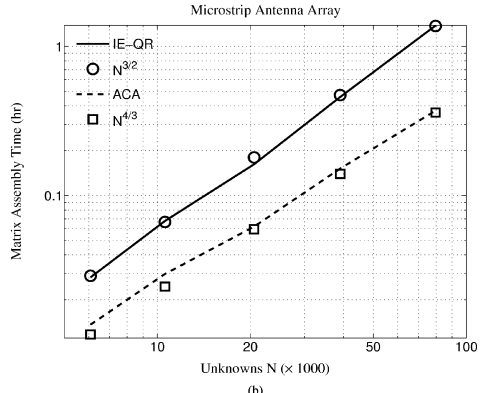
\includegraphics[width=\linewidth]{zhoa_time_assembly.png}
	\captionsetup{justification=centering}
	\caption{Comparisons of the complexity between ACA and single-level IE-QR algorithms for layered medium application (CPU time). All the computations were performed on a Pentium IV 1.8 GHz with 2 GB RAM PC \cite{zhao_adaptive_2005}}
	\label{fig:zhoa_time_assembly}
\end{figure}

Sur ce graphique on remarque que la ACA (Figure \ref{fig:zhoa_time_assembly}) suit une complexité de $\mathcal{O}(Nlog(N))$ à fréquence fixe. Ce résultat est meilleur que le pire cas théorique que l'on a présenté et peut donc convenir. Toutefois, on sait que le comportement asymptotique de la ACA n'est plus suffisant en complexité \cite{tamayo_multilevel_2011}.

\subsubsection{Erreurs}
Ce qui fait aussi que de meilleurs algorithmes sont recherchés sont les erreurs lors de l'approximation par compression de la matrice $M$. Elle permet de gagner en espace de stockage au détriment de la précision. \cite{zhao_adaptive_2005}.

\begin{figure}[ht]\centering
	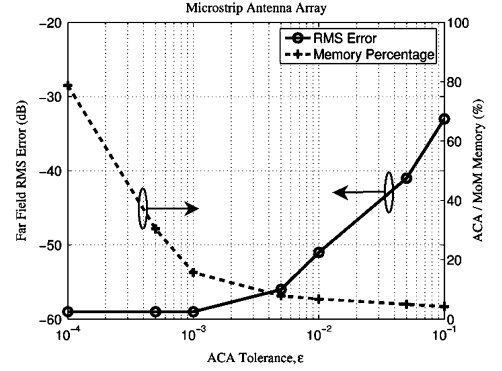
\includegraphics[width=\linewidth]{zhao_tolerance_ACA.png}
	\captionsetup{justification=centering}
	\caption{Far-field rms error and ratio between memory for ACA and memory for MoM as a function of ACA terminating tolerance $\epsilon$. The study is performed with a 8 × 8 corporate-fed microstrip array \cite{zhao_adaptive_2005}}
	\label{fig:zhao_tolerance_ACA}
\end{figure}

Sur ce graphique ( Figure \ref{fig:zhao_tolerance_ACA}) qui représente la mémoire en fonction de la précision demandé, on voit bien que malgré la compression, le modèle de l'utilisation mémoire est exponentiel avec la monté en précision. L'algorithme est donc gourmand en erreur et fourni des erreurs de résolution. Il es donc intéressant de se tourner vers une autre solution d'algorithme de résolution rapide qui se base sur la ACA.

\subsection{La MLACA}
\subsubsection{Présentation de l'algorithme}
La MLACA est un autre algorithme algébrique qui sert à résoudre des équations comme des couplages magnétiques, ou des forces à l'intensité décroissante avec la distance \cite{nel_efficient_2019}. L'objectif est d'approximer des parties du calcul selon la distance auxquels les éléments se trouvent les uns des autres. On se figure une matrice $L$, l'ensemble des couples entre deux éléments $(i,j)$, telle que :

\begin{equation}
    L[i,j]= \frac{\mu}{4\pi a_i a_j} \int_{V_i} \int_{V_j}\frac{\hat{l}_{i} \, \hat{l}_{j}}{|r_i - r_j|}dV_i dV_j 
\end{equation}

Ensuite, au lieu de calculer exactement la force qui s'applique, on définis un critère de champs lointain autour de notre observateur qui va servir de bordure à l'approximation des champs lointains. Comme on le voit représenté sur ce grraphique (Figure \ref{fig:far_neighbor}) tiré du travail de Ben A.P. Nel \cite{nel_mlaca_2019} :

\begin{figure}[ht]\centering
	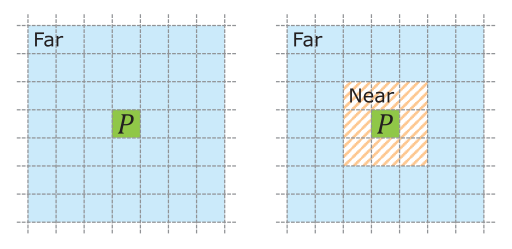
\includegraphics[width=\linewidth]{far_neighbor.png}
	\captionsetup{justification=centering}
	\caption{fig:Two near-interaction criteria, with respect to observer group P. Left: self interaction criterion. Right: nearest-neighbor criterion \cite{nel_efficient_2019}}
	\label{fig:far_neighbor}
\end{figure}

On comprend intuitivement que l'approximation d'un groupe d'éléments qui interagissent avec l'observateur comme un unique corps permet de diminuer la demande en calcul \cite{nel_efficient_2019}. Cet algorithme par niveaux donne donc une compression de notre matrice $M$ en divisant la fonction de base. On rappelle que cet algorithme est basé sur le fait que le degré de liberté reste asymptotiquement le même. Un niveau $P$, de la MLACA, divise les fonctions de base de la ACA ; un niveau se subdivise alors en $2^P$ \cite{gibson_efficient_2020} auxquels on applique l'algorithme du papillon dans lequel les sous-groupes sont récursivement fusionnés et séparés avec une ACA appliquée à chaque niveau. Cet algorithme récursif permet de calculer des ensembles de matrices qui se subdivisent à chaque niveau. On voit bien sur la représentation ( Figure \ref{fig:mlaca_paralel}) de la compression des matrices par multi niveaux  que la compression de la matrice peut se calculer indépendemment en blocs eux même compressé et tiré du travail de Walton C. Gibson \cite{gibson_efficient_2020} :

\begin{figure}[ht]\centering
	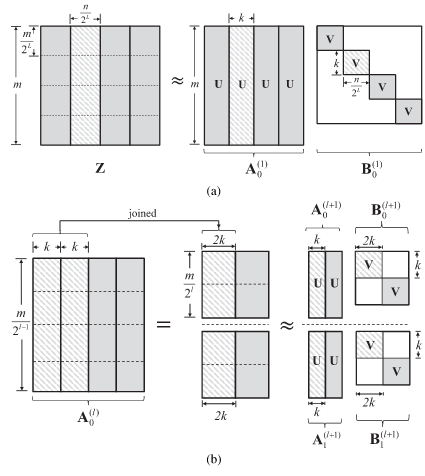
\includegraphics[width=\linewidth]{mlaca_paralel.png}
	\captionsetup{justification=centering}
	\caption{2-Level U -type MLACA. (a) Operations on level l = 0. (b) Operations on level l + 1 \cite{nel_mlaca_2019}}
	\label{fig:mlaca_paralel}
\end{figure}

C'est pourquoi cet algorithme est si facilement parallélisable. Par la MLACA on peut facilement approximer notre matrice par compression. Toutefois, il faut faire attention lors du découpage par bloc à ne pas calculer plusieurs fois les mêmes parties. De même, il y a un ordre dans lequel calculer ces sous-groupes de façon optimisée \cite{tamayo_multilevel_2011}.

\subsubsection{Analyse du coût}
Tout d'abord, le coût de stockage de la MLACA se trouve presque intuitivement en sachant qu'à chaque niveau on divise par 2 notre matrice. On arrive rapidement à ue complexité :$\mathcal{O}(N+Nlog(N)) \, \approx \, \mathcal{O}(Nlog(N))$ \cite{tamayo_multilevel_2011}.

D'autre part pour le coût de calcul, s'obtient en sachant que l'on effectue $2^P$ ACA (avec $P$ le nombre de niveau de la MLACA) sur des matrices de rang $k$ et de dimension $m \times n \, / \, (2^P)$. Il faut en plus à chaque étape effectuer une décomposition par ACA sur une matrice de même rang mais de dimension $(m / 2^i) \times 2k$. L'ensemble de ces opérations donne un coût total de complexité $\mathcal{O}(N^2)$ \cite{tamayo_multilevel_2011}.

La MLACA étant implémenté dans le projet GitHub ERCEM321\textunderscore ATREYU \cite{git_proj}, des tests ont été effectués pour voir son comportement asymptotique selon la taille de la matrice et la précision demandée. 

\begin{figure}[ht]\centering
	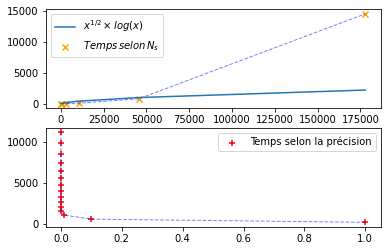
\includegraphics[width=\linewidth]{Atreyu_test.png}
	\captionsetup{justification=centering}
	\caption{Benchmark effecuté depuis le projet GitHub \cite{git_proj}}
	\label{fig:atreyu_test}
\end{figure}

Ce graphique (Figure \ref{fig:atreyu_test}) met en avant deux choses :
\begin{itemize}
    \item[$\bullet$] L'implémentassions de la MLACA dans le projet GitHub possède une meilleure complexité que la MLACA classique car modèle qui lui correspond le plus est une complexité de $\mathcal{O}(N^{1/2} \times log(N))$ qui est loin de la complexité en $\mathcal{O}(N^2)$ dont on parlait précédemment. Mais malgré cette amélioration on observe une explosion du temps de calcul. Cette explosion s'explique par le temps que mettent les informations pour transiter de coeur à coeur \cite{nel_efficient_2019}. Ce transfert de donnée fait perdre du temps à l'algorithme. De plus à cause de ce transit, tous les coeurs ne travaillent pas toujours, comme on le voit sur cette capture (Figure \ref{fig:htop}) lors de la compilation du code de MLACA. 
    
    \begin{figure}[ht]\centering
	    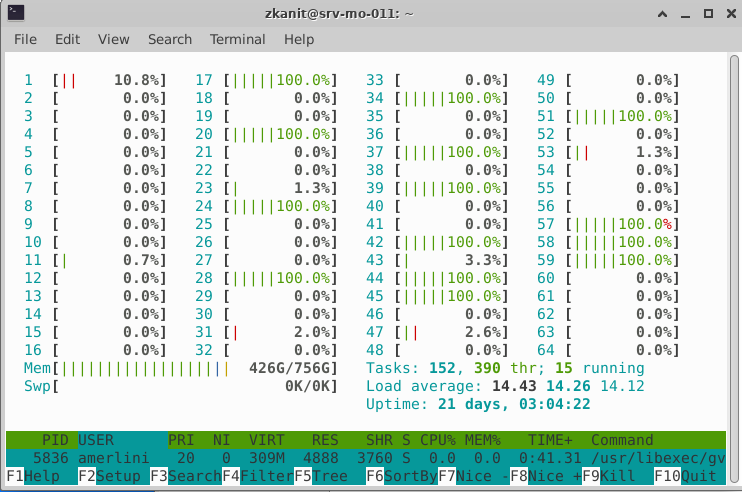
\includegraphics[width=\linewidth]{htop.png}
    	\captionsetup{justification=centering}
    	\caption{Activité des coeurs pendant la MLACA}
    	\label{fig:htop}
    \end{figure}
    
    \item[$\bullet$] Le temps en fonction de la précision croit quant à lui de façon plus que exponentielle. La tolérance est donc un paramètre qui encore une fois décuple le temps de travail de l'algorithme quoi que l'on fasse. Malheureusement, ce temps de travail cumulé aux erreurs de compression comme on l'a vu sur la ACA nécessitent la recherche de solution qui conviendrait mieux à la situation.
\end{itemize}

La MLACA est donc un algorithme très puissant, mais malheureusement, se sont les limites techniques du transfert de données qui l'empêchent de déployer tout son potentiel. Cherchons si l'approximation par bloc peut résoudre ces problème. 

%------------------------------------------------

\section{Approximation par blocs (BACA)}
\subsection{Algorithme}
L'algorithme de BACA dérive directement de la ACA. Au lieu, de choisir une unique colonne et ligne pour compresser la matrice, on choisit maintenant un groupe fini de lignes et colonnes pour obtenir la relation (\ref{eq:BACA_compression}) \cite{liu_parallel_2020} :

\begin{equation}
    M \, \approx \, UV \, = \, \sum_{k=1}^{n_j} U_kV_k 
    \label{eq:BACA_compression}
\end{equation}

Avec $U_k \, \in \, \mathbb{R}^{m \times d_k}$ et $V_k \, \in \, \mathbb{R}^{d_k \times n}$. 

Normalement, l'algorithme choisit des valeurs de pivot de façon aléatoire ou optimisée. Mais pour performer la BACA, les pivot $(i_k,j_k)$ sont choisis grâce à une décomposition QR préalable\cite{liu_parallel_2020} sur les transposées des $d_k<d$ colonnes. Nous allons présenter les 3 étapes de chaque étape de la BACA avant d'en proposer un algorithme :
\begin{enumerate}[noitemsep] % [noitemsep] removes whitespace between the items for a compact look
    \item Trouver le bloc de lignes $I_k$ et le bloc de colonnes $J_k$ par décomposition QR \cite{ros_code} en commencant par $J_1$ de façon aléatoire, puis en appliquant l'algorithme :
    \begin{equation}
        (Q_k^c,T_k^c,I_k)=\mathbf{QR}(R_{k-1}[:,J_k]^t,d),I_k
    \end{equation}
    \begin{equation}
        (Q_{k+1}^c,T_{k+1}^c,J_{k+1})=\mathbf{QR}(R_{k-1}[I_k,:],d),J_k
    \end{equation}
    L'algorithme choisit les blocs à partir des sous matrices $R_k$ $R_{k-1}$. Pour se faire, l'implémentation de la décomposition $\mathbf{QR}$ sur Rosetta Code a été utilisé \cite{ros_code} et qui choisit le pivot en recherchant des le coefficient maximal dans la colone de la décompositon $\mathbf{QR}$. 
    A noter que pour avoir un résultat optimal il est préférable de prendre $d$ lignes et colonnes \cite{liu_parallel_2020}. De plus, il faut éviter d'utiliser sur plusieurs itérations les mêmes lignes; c'est pourquoi la décomposition $\mathbf{QR}$ est faite  sur une sous-matrice de $R_{k-1}[:,J_k]^t$ plutôt que directement sur $R_{k-1}[:,J_k]^t$. Bien sûr on fait de même avec $R_{k-1}[I_k,:]$. Pour comprendre cette étape, il est possible d'utiliser le schémas (Figure \ref{fig:schemas})
    
    \begin{figure}[ht]\centering
	    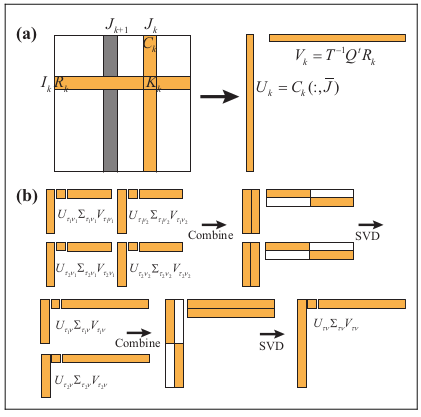
\includegraphics[width=\linewidth]{schemas.png}
    	\captionsetup{justification=centering}
    	\caption{(a) Selection of I_k/J_k and form the low-rank update U_kV_k. (b) Low-rank merge operation}
    	\label{fig:schemas}
    \end{figure}
    \item Ensuite, on forme les facteurs de bas rang produit de $U_kV_k$. Par exemple avec $C_k=R_{k-1}[:,J_k], \, \mathbf{R}=R_{k-1}[I_k,:]$ et $W_k=R_{k-1}[I_k,J_k]$. On trouve la relation $R_{k-1} \approx C_k W_k^T \mathbb{R}_k=U_k V_k$. A noter que la matrice $W_k$ est souvent en déficit de rang. Dans ce cas, la BACA devient beaucoup plus puissante que la ACA avec $d_k$ pivots et peut être utilisée pour générer $d$ colonnes $J_{k+1}$ pour l'itération suivante.
    
    On met alors à jour les pivots $(I_k,J_k)$ dans la relation (\ref{eq:BACA_update}) par le pivot $\overline{J}$ obtenu par décompoosition $\mathbb{QR}$.
    \begin{equation}
        (Q,T,\overline{J})=\mathbf{QR}(W_k=R_{k},\epsilon)
    \end{equation}
    \begin{equation}
        U_k=C_k[:,\overline{J}], \, V_k=T^{-1}Q^t\mathbf{R_k}
    \end{equation}
    \begin{equation}
        I_k \longleftarrow I_k[1:d_k], \, J_k \longleftarrow J_k[\overline{J}]
        \label{eq:BACA_update}
    \end{equation}
    \item Ensuite il faut calculer $\nu=||U_kV_k||_F$ et mettre à jour $\mu=||UV||_F$ en supposant que la mise à jour de la valeur du bas rang de dimension $d \times d$ soit de complexité $\mathcal{O}(nd_k^2)$ par l'opération :
    \begin{equation}
        T_{U_k}= Chol(U_k^t U_k), \, T_{V_k}=Chol(V_k V_k^t)
    \end{equation}
    \begin{equation}
        \nu = || T_{U_k} T_{V_k}^t||_F
    \end{equation}
    Puis la mise à jour de la valeur de la norme de $UV$ en $\mathcal{O}(n r_k d_k)$.
    \begin{equation}
        \mu^2 \longleftarrow \mu^2+\nu^2+2\sum_{i=1}^{r_{k-1}} \sum_{j=1}^{d_k} \Tilde{V}[i,j]
    \end{equation}
    On obtient donc le vecteur :
    \begin{equation}
        \Tilde{V}=(V V_k^t) \circ (U^tU_k)
    \end{equation}
    On peut noter qu'une valeur de $d$ plus grande permet de donner une meilleure approximation à notre compression \cite{liu_parallel_2020}. Pour le pseudcode de l'algorithme.
\end{enumerate}
\begin{algorithm}
    \caption{Blocked Adaptive Cross Approximation}
    
    \KwInput{$M \, \in \, \mathbb{R}^{m \times n},d \, \in \, \mathbb{N}, \epsilon \text{ tolérance}$}
    \KwOutput{Approximation à bas rang $r$ de $M \approx UV$}
    
    $U \, = \, 0, \, V \, = \, 0, \, \mu \, = \, 0, \, r_0 \, = \, 0, \, J_1 \, \text{liste de d index aléatoire}$
    
    \For{$k=1 \text{ to min($m,n$)}$}{
        $C_k=R_{k-1}[:,J_k]$
        $(Q_k^c,T_k^c,I_k)=\mathbf{QR}(C_k^t,d),I_k$
        $\mathbf{R}_k = R_{k-1}[I_k,:]$
        $(Q_{k+1}^r,T_{k+1^r}, J_{k+1})=\mathbf{QR}(R_k,d),J_{k+1}$
        $W_k=R_{k-1}[I_k,J_k]$
        $(U_k,V_k,d_k,\overline{J})=LRID(C_k,W_k,R_k,\epsilon)$
        $I_k \longleftarrow I_k[1:d_k], \, J_k \longleftarrow J_k[\overline{J}]$
        $r_k = r_{k-1}+d_k$
        $\nu = LRnorm(U_k,V_k)$
        $\mu \longleftarrow LRnormUp(U,V,\mu,U_k,V_k,\nu)$
        $U \longleftarrow (U,U_k), \, V \longleftarrow (V, V_k)$
        $\text{Return if } \nu < \epsilon\mu$
        }
        
    \SetKwProg{Fn}{Def}{:}{}
    \Fn{LDIR(C,W,R,\epsilon)}{
        $(Q,T,\overline{J}, r)= \mathbf{QR}(W, \epsilon) $\;
        $U=C[:,\overline{J}] $\;
        $V=T^{-1}Q^tR $\;
        $\text{Return } U,V,r,\overline{J}$
    }
    
    \SetKwProg{Fn}{Def}{:}{}
    \Fn{LRnorm(U,V)}{
        $T_1=Chol(U^t U) $\;
        $T_2=Chol(V V^t) $\;
        $\text{Return }||T_1T_2^t||_F $
    }
    
    \SetKwProg{Fn}{Def}{:}{}
    \Fn{LRnormUp(U,V,\nu,\overline{U},\overline{V},\overline{\nu})}{
        $s=\nu^2+\overline{\nu}^2+2\sum_{i=1}^{r_{k-1}} \sum_{j=1}^{d_k} \Tilde{V}[i,j]$\;
        $\Tilde{V}=(V V_k^t) \circ (U^tU_k)$\;
        $\text{Return }\sqrt{s}$
    }
\end{algorithm}


Le fait que BACA prennent des blocs entiers permet une convergence plus rapide et peut aussi être amélioré par le choix de bons critères d'arrêts \cite{liu_parallel_2020}.
Une fois encore la compression se fait sans a-priori sur le coeur, on peut donc appliquer cette méthode sur à peu près à toutes les fonctions de Green.
Ce compactage en bloc permet à ce que certaines opérations deviennent "BLAS-3" par ce processus; c'est à dire que les types ainsi que leur opérations élémentaires sur la carte mère sont adaptées à l'utilisation sur un seul processeur avec plusieurs coeurs. Cette situation convient donc parfaitement à l'usage que l'on veut faire de cet algorithme.

Le choix d'un $d$ judicieux affectera la balance entre efficacité et véracité. 

\subsection{Parallélisation}
Cet algorithme du fait de sa computation par blocs peut facilement se répartir sur différents coeurs afin de paralléliser le calcul \cite{liu_parallel_2020}. Il faut alors hiérarchiser le grillage de surface, mais cette opération se fait sans grande difficulté avec les outils présents dans le projet GitHub \cite{git_proj}. Ensuite, pour mettre en oeuvre la parallélisation, il suffit de faire faire le BACA à un processeur pendant que deux autres gèrent deux calculs de sous-matrices avant de fusionner ces matrices de bas rang.

\subsection{Analyses du coût}
La nature à travailler par bloc de la BACA en fait un algorithme de choix en terme de complexité. Cela permet d'utiliser de moins nombreux pivots qui montre une convergence continue et presque assurée. De plus l'opération par bloc bénéficie de la haute performance des flip-flop en "BLAS-3".
On peut donc penser que la complexité originellement en $\mathcal{O}(Nr^2)$ est peut être meilleure. Il faudrait prendre en compte le calcul des sous matrices qui aurait une complexité en $\mathcal{O}(\sqrt{n_b})$, mais à moins d'avoir un $n_b$ qui dépende de la taille de la matrice, la complexité du BACA est la même que celle de la ACA puisqu'elle est asymptotiquement $\mathcal{O}(nr^2\sqrt{n_b})$; du moins en théorie \cite{liu_parallel_2020}.

En pratique, la "BLAS-3" permettrait une hausse des performances considérable \cite{liu_parallel_2020}.

%------------------------------------------------

\section*{Conclusion}

\addcontentsline{toc}{section}{Conclusion} % Adds this section to the table of contents

Nous n'avons malheureusement pas pu voir avec notre propre algorithme avec des résultats. Cependant, nous pouvons voir que le développement de la BACA apporte une solution algébrique efficace aux problèmes de résolution d'équation. La BACA tiend sa force au fait d'utiliser le principe de la ACA sur des blocs, ce qui la rend d'autant plus robuste et efficace. Malheureusement, aggrandir la taille des blocs peut se trouver être un risque jusqu'à un certain point qu'il faudrait déterminer expérimentalement.

Il existe encore des façons d'améliorer la BACA ; la parallélisation requiert de faire attention à la distribution des données, car puisque BACA précède la MLACA, la réflexion sur le coût de communication est une réflexion à avoir en tête pour de futurs améliorations.

%------------------------------------------------

\section*{Remerciements} % The \section*{} command stops section numbering

\addcontentsline{toc}{section}{Remerciements} % Adds this section to the table of contents

Je tiens à remercier M.Merlini qui a pris de son temps pour encadrer et expliquer ce projet ; les concepts théoriques et mathématiques qui soutiennent ces algorithmes. Ainsi que Clément Henry qui a aussi pris de son temps de travail pour m'expliquer le fonctionnement du projet et la connection au serveur.

Je remercie Benjamin Somers de m'avoir fourni un serveur puissant lorsque l'autre n'était pas accessible.

%----------------------------------------------------------------------------------------
%	REFERENCE LIST
%----------------------------------------------------------------------------------------

\bibliographystyle{unsrt}
\bibliography{bibli_CODEV}

%----------------------------------------------------------------------------------------

\end{document}